\chapter{Einzelansicht Mitglied}\label{personal:person}
Das Fenster in \cref{fig:personal:person} zeigt das Standardfenster für die Bearbeitung der Personendaten.
Im Kopf werden der Name und die Mitgliedsnummer angezeigt und können geändert werden.
Beim Erstellen einer Person wird automatisch, die nächsthöhere Mitgliedsnummer vergeben, als aktuell vorhanden.
Ein Ändern der Mitgliedsnummer ist nur möglich, wenn die Nummer nicht bereits vergeben ist.

Für juristische Personen, die als Fördermitglieder aufgenommen sind, kann der Vorname freigelassen werden.
Es genügt hierbei den Nachnamen anzugeben.

\begin{figure}[!h]
  \centering
	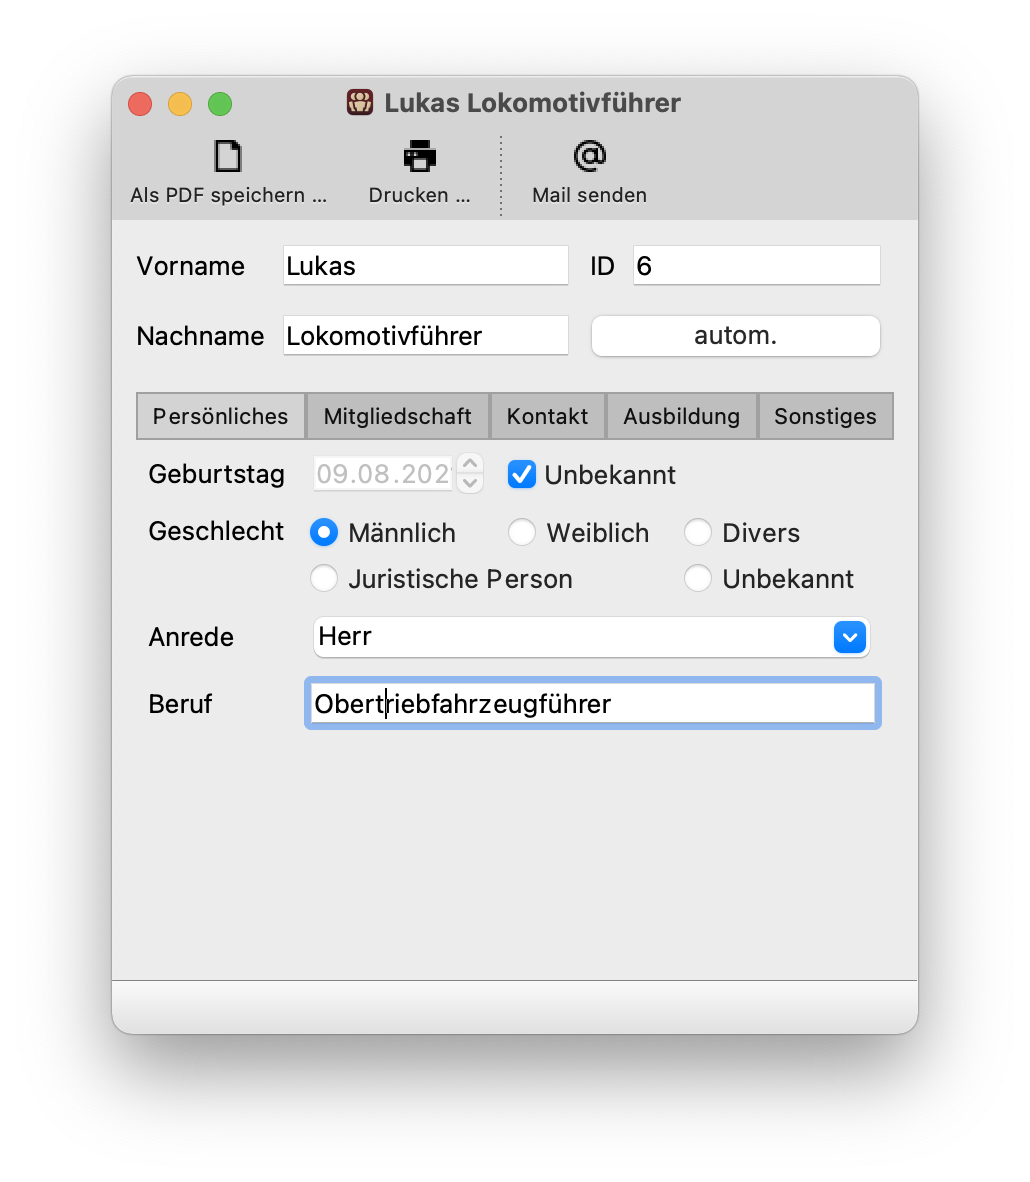
\includegraphics[width=0.75\textwidth]{img/personal-person}
	\caption{Das Fenster zum Bearbeiten der Daten eines Mitglieds.}
	\label{fig:personal:person}
\end{figure}


Im unteren Bereich des Fensters stehen verschiedene Reiter zur Verfügung,
über welche die persönlichen Daten abgerufen und verändert werden können.

\paragraph{Persönliches.}
Hier können verschieden persönliche Daten des Mitglieds angepasst werden.
Dies umfasst unter anderem das Geschlecht, Beruf, Alter und Anrede.

\paragraph{Mitgliedschaft.}
Hier können die Rahmendaten der Mitgliedschaft geändert werden.
Dies sind vor allem das Eintrittsdatum und der Status (aktiv oder passiv).
Ebenso kann die Art des Beitrags eingestellt werden
und die Daten der Bankverbindung.
Bei einer Familienmitgliedschaft (bzw.\ beim Nutzer) wird unter Kontoinhaber (bzw. dann Zahler)
der Name des Mitglieds angegeben, dass den Familienbeitrag zahlt.
Dort ist dann als Beitragsart "`Familienbeitrag (Zahler)"' zu wählen.
\begin{neu}
Im Feld Beitrag wird der Beitrag der Person angezeigt.
Eine eventuelle weitere Angabe in Klammern gibt die Höhe der aktuell anstehenden Nachzahlungen an,
die auf nicht erbrachten Pflichtstunden basieren.
Dieser Wert kann sich ändern, wenn die Person in Aktivitäten im \Einsatz eingetragen wird.
Wird kein Wert angegeben, hat die Person ihre Pflichtstunden erfüllt
oder es fallen keine solchen an.
Siehe \cref{personal:mitglieder:beitrag} für weitere Informationen.
\end{neu}

\paragraph{Kontakt.}
Hier besteht die Möglichkeit eine Postadresse (Wohnort)
und E-Mail-Adresse und Telefonnummern anzugeben.
Ebenso kann hier die Entfernung zum Bahnhof eingestellt werden.

\paragraph{Ausbildung.}
Für den Betriebsdienst kann ein Datum eingegeben werden, dass beschreibt bis wann die betriebliche Tauglichkeitsuntersuchung gültig ist.
Ebenso kann die Qualifikation angegeben werden.
Liegt für den Tag einer Aktivität keine Tauglichkeit vor,
kann die Person nicht in der entsprechenden Kategorie eingetragen werden
(z.B.\ als Tf oder Zf).
Für Zugbegleiter wird dann automatisch eine Eintragung als Begl.o.b.A.\ eingetragen.
Darüber hinaus können weitere betriebliche Bemerkungen angegeben werden
sowie nicht-betriebliche Ausbildungen und Qualifikationen.

\paragraph{Sonstiges.}
Hier finden sich zwei Felder bezüglich des Datenschutzes,
um einen Sperrvermerk für Telefonnummern oder Mail-Adressen zu hinterlegen.
Ein Feld für Bemerkungen erlaubt es beliebigen Freitext einzugeben.



\paragraph{Person Löschen}
Sie können über das Menü \aktion{Person} die Person aus dem System entfernen.
Dies ist nur möglich, wenn sie bei keiner Aktivität mehr eingetragen ist.
Ist eine Person aus dem Verein ausgetreten, ist es \textbf{nicht} erforderlich sie zu löschen.
Stattdessen kann die Person im Reiter \button{Mitgliedschaft} als ausgetreten markiert und das Austrittsdatum vermerkt werden.
Somit bleibt die Person weiterhin im System erhalten und wird auch bei den jeweiligen Aktivitäten noch mit ausgegeben.


\paragraph{Export}
Über das Menü \aktion{Export} kann das Stammdatenblatt der geöffneten Person exportiert werden.
Das Dokument enthält alle personenbezogenen Daten aus der EPL-Datei.
Es enthält jedoch keine Informationen zu Aktivitäten und geleisteten Stunden.
